\chapter{Introduction}

\section{Motivation}
Revealing the structure of hierarchical organized data is a complex task where many approaches already exists (TODO cite). It is still an active research area as data scientists are facing ever greater challenges when analyzing large hierarchical datasets. One example is the Human Disease Network \cite{zhou_human_2014} which is a hierarchical network of disorders and disease genes with approximately 3000 nodes on two different hierarchy layers. Figure \ref{fig:Human_Disease_Network} shows us the representation of the data in a common two-dimensional layout where the classes of disorders are color coded. 
Our own dataset which also contains a similar structure can be seen in Figure \ref{fig:original2DdiseaseNet}. Here the clusters of different diseases are grouped by boxes. Depiction of hierarchical network structure in 2D faces us with many challenges: limitation of visual features, only two available axes for encoding spatial data and therefore limiting the ability of the user to detect clusters and lastly visualizing more than two layers. However, in other application areas like software engineering or social science we often face more than two hierarchical layers, so we need to find a way to handle these datasets. 

\begin{figure}[h]
    \centering
    \begin{subfigure}[b]{0.4\columnwidth}
        \centering
        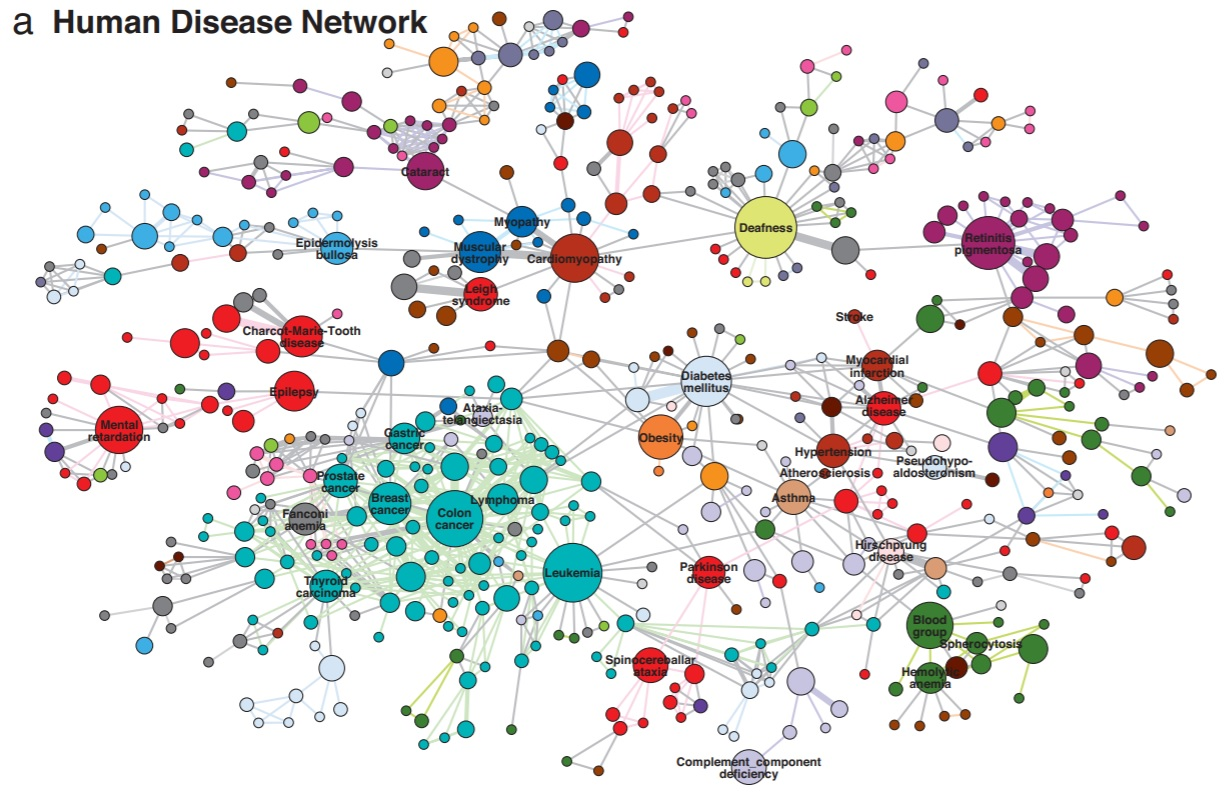
\includegraphics[width=\textwidth, trim={0 0 9cm 0},clip]{graphics/Human_Disease_Network.jpg}
        \subcaption{Human Disease Network \cite{zhou_human_2014}}
        \label{fig:Human_Disease_Network}
    \end{subfigure}
    \begin{subfigure}[b]{0.5\columnwidth}
      \centering
      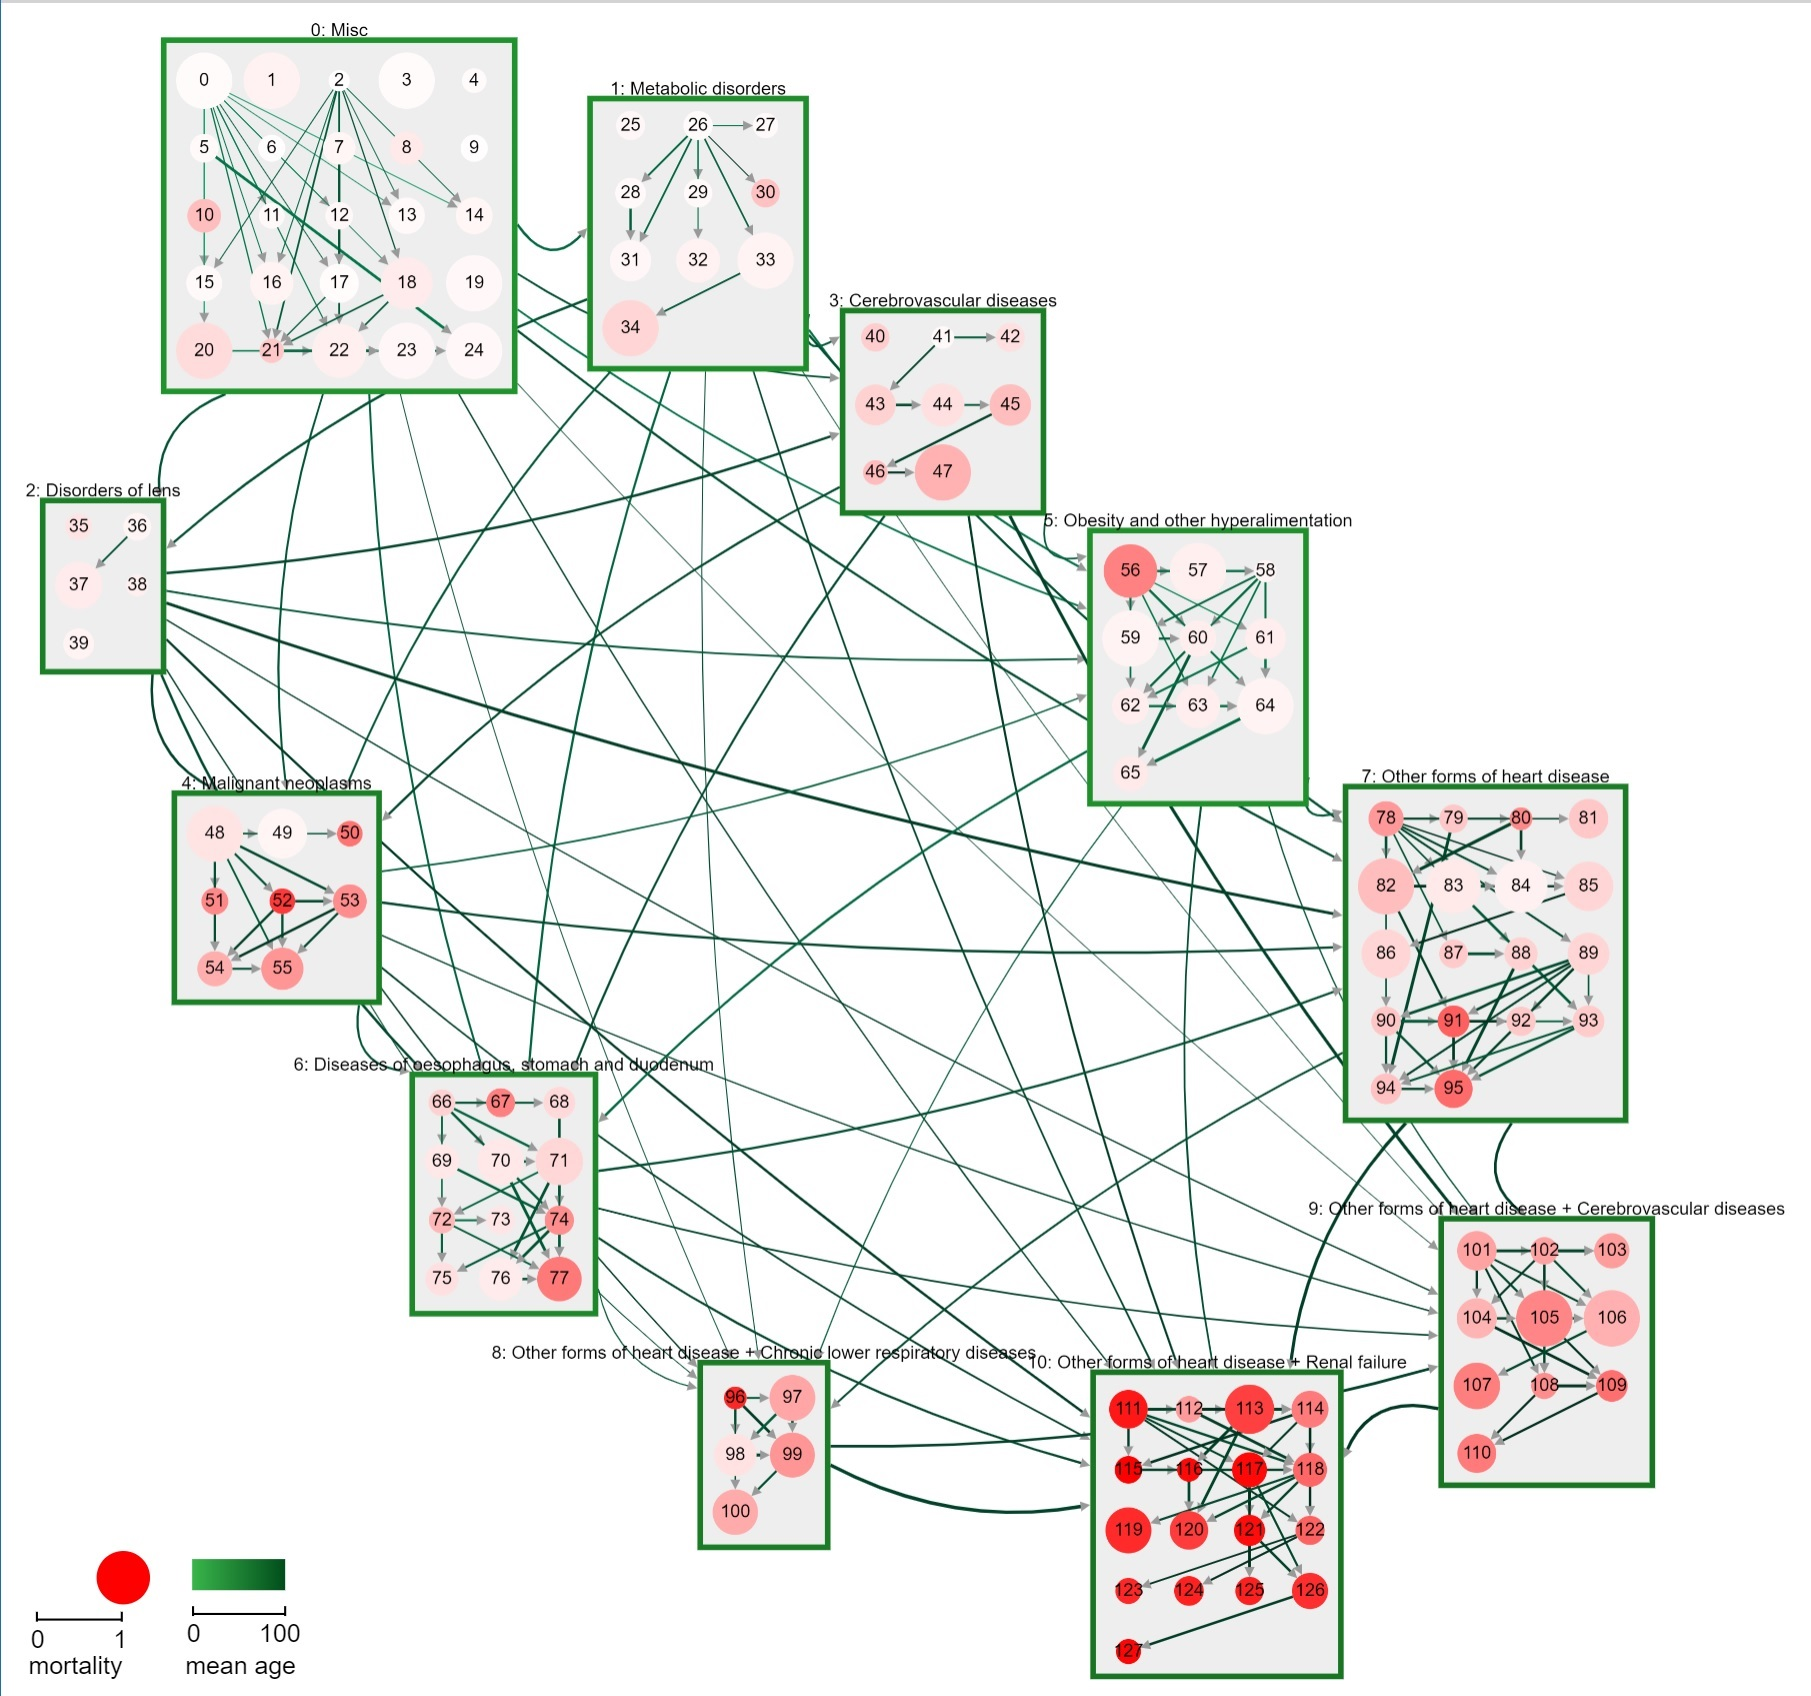
\includegraphics[width=\textwidth]{graphics/original2DdiseaseNet.jpg}
      \subcaption{Our own disease network dataset}
      \label{fig:original2DdiseaseNet}
    \end{subfigure}
    \caption[Optional caption for the figure list (often used to abbreviate long captions)]{Example visualizations of hierarchical network datasets in two dimensions. Both consists of two hierarchical layers.} % Remove the [...] argument if the original caption should be used in the figure list.
    \label{fig:intro} 
  \end{figure}

3D information visualization allows us to expand the user experience of traditional 2D graphs. As Brath describes in his paper \cite{brath_3d_2014} there are many advantages and opportunities when using three-dimensional visualizations.
An obvious one would be that we can encode more spatial information by using an additional axis. A good example therefore is the “3D space time cube” which displays the temporal information on the Z axis, another common would be a 3D scatter plot. By using these additional spatial information the mental model of the data gets improved which results in a better understanding by the user.
In the context of visual features we get a lot more of opportunities, one of the biggest is probably the ability to use surfaces and effects like shading. 
The view on the visualization can be reconsidered in a three-dimension context. Usually the user looks from the outside at visualization. In 3D however the viewer can be placed right inside our graph, this enables us to utilize new navigation and interaction possibilities. 

Naturally all these opportunities entails new challenges in navigation in the graph, occlusion of elements in an 3D perspective view, selection for displaying details and the lack of a reference point in three-dimensional space. Brath \cite{brath_3d_2014} already said that immersive interfaces could help to overcome this issues. We believe that with the recent developments in virtual reality hardware and frameworks these challenges can not be better solved. Bowman et al. \cite{bowman_virtual_2007} already research the impact of VR techniques like stereoscopic images, interaction with the virtual world and head movement can have on users. Recently Kraus et al. \cite{kraus_impact_2020} did a study where they examined the effect of immersion for detecting clusters in a scatter plot. Their results shows that VR based visualization systems have real world advantages in terms of time needed to get an overview of the data compared to traditional 2D- and 3D information visualization. In terms of navigation Yang et al. \cite{yang_embodied_2020} and Drogemuller \cite{drogemuller_examining_2020} presented some techniques.  

%Data scientists are facing ever greater challenges when analyzing large datasets with a hierarchical structure. 

%From proposal: \\
%The	 goal	 is	 to	 visualize	 a	 hierarchical	 network	 with	 n	 Layers.	 Each	 Node	 in	 a	 graph	 can	
%represent	a	graph	itself.	There	are	multiple	examples	where	this	has	been	visualised	in	2D,	
%however	we	believe	that	with	an	additional	dimension	and	when	3D	graphs	are	analysed	in	
%VR	we	can	get	even	more	insight	and	a	better	overview	of	the	data.	

\textbf{Starting idea: 2D Multilayer see figure, why not make use of all 3 axes in VR, instead of flat layers use 3D objects like cubes/spheres to bundle one layer} (Email 14.08.2020 https://arxiv.org/pdf/1902.06815.pdf)
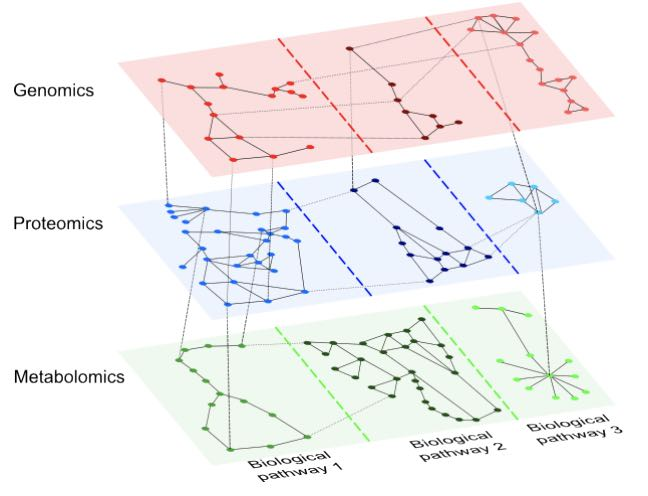
\includegraphics[width=0.5\textwidth]{chapters/graphics/2dmultilayerVis.jpg}

Ideas:
\begin{itemize}
    \item Example applications with hierarchical network data
    \item current 2D visualizations of hierarchical networks
    \item power of VR visualizations and board availability
\end{itemize}

\section{Aim of the Work}

Ideas:
\begin{itemize}
    \item provide a prototype application
    \item benefits of webbased implementation 
    \item experiment with different concepts/approaches
    \item experiment with different interactions
    \item ...
\end{itemize}

\begin{quotation}
    However, there is considerable value in research that
    solves a well-motivated problem using a combination
    of preexisting solutions 
\end{quotation}
Sadana\\
Redefining a Contribution for Immersive Visualization Research\\

\section{Approach}

I want to give a short summary of chapter 4 proposed solution here. 

Ideas:
\begin{itemize}
    \item short description of planned final solution (web based, htc vive compatible, rendering multi hierarchical dataset, screenshot of solution)  
    \item short overview of used technologies and frameworks why? what it simplifies, ... 
    \item Customized Forces
    \item rendering, nodes inside parent, comparison to a default 2D Circle Packing plot https://observablehq.com/@d3/zoomable-circle-packing 
    \item available interactions
\end{itemize}